\documentclass[11pt, a4paper]{article}

% Fonts and Encoding
\usepackage[utf8]{inputenc}
\usepackage[T1]{fontenc}

% Math and Symbols
\usepackage{amsmath, amssymb, amsthm, amsfonts, mathrsfs, mathtools}

% Layout and Geometry
\usepackage{geometry}
\geometry{a4paper, margin=1in}

% Formatting and Graphics
\usepackage{graphicx, xcolor, enumitem, booktabs, array, tabularx}

% TikZ for Illustrations
\usepackage{tikz}
\usetikzlibrary{arrows.meta, positioning, shapes.geometric, calc, backgrounds, matrix}

% Clickable Links and TOC
\usepackage{hyperref}
\hypersetup{
    colorlinks=true,
    linkcolor=blue,
    filecolor=magenta,      
    urlcolor=cyan,
    pdftitle={Mathematical Induction: Foundations and Applications},
}

% Theorem Environments
\newtheorem{theorem}{Theorem}[section]
\newtheorem{lemma}[theorem]{Lemma}
\newtheorem{proposition}[theorem]{Proposition}
\newtheorem{corollary}[theorem]{Corollary}
\theoremstyle{definition}
\newtheorem{definition}{Definition}[section]
\newtheorem{axiom}{Axiom}[section]
\newtheorem{example}{Example}[section]
\theoremstyle{remark}
\newtheorem{remark}{Remark}[section]

% Custom Commands (Enforced standard notation)
\newcommand{\R}{\mathbb{R}}
\newcommand{\N}{\mathbb{N}}
\newcommand{\Z}{\mathbb{Z}}
\newcommand{\Q}{\mathbb{Q}}
\newcommand{\E}{\mathbb{E}}
\newcommand{\Prob}{\mathbb{P}}
\newcommand{\F}{\mathcal{F}}

\begin{document}

\title{\textbf{Mathematical Induction: Foundations and Applications}\\ \Large Rigorous Proofs, Set-Theoretic Foundations, and Quantitative Modeling}
\author{Tashfeen Omran}
\date{\today}

\maketitle
\tableofcontents
\newpage

% ==========================================
% PART 1: INTRODUCTION
% ==========================================
\section{Comprehensive Introduction, Context, and Prerequisites}

\subsection{Core Concepts \& Axioms}
Mathematical Induction is not merely a technique for algebraic verification; it is a profound foundational axiom of the natural numbers, $\N$. At its core, induction provides a rigorous mechanism to transition from the finite to the countably infinite. When we wish to prove that a property $P(n)$ holds for all $n \in \N$, we are essentially attempting to map the entire set of natural numbers to the Boolean value of ``True''. 

The formalization of this process relies on the \textbf{Well-Ordering Principle (WOP)}, which states that every nonempty subset of the positive integers contains a least element. From this seemingly simple set-theoretic property, the Principle of Mathematical Induction (PMI) is derived. 

\subsection{Intuition and Set-Theoretic Foundations}
Imagine an infinite sequence of dominoes. To guarantee that every domino falls, two conditions must be met:
\begin{enumerate}
    \item You must knock over the first domino (The \textbf{Base Step}).
    \item The spacing between the dominoes must be such that if any arbitrary domino $k$ falls, it inevitably knocks over domino $k+1$ (The \textbf{Inductive Step}).
\end{enumerate}
Set-theoretically, let $S$ be the set of all $n \in \N$ for which $P(n)$ is true. The base step shows $1 \in S$. The inductive step shows that if $k \in S$, then $k+1 \in S$. By the axioms of Peano arithmetic, this implies $S = \N$. If $S \neq \N$, the complement $\N \setminus S$ would be a nonempty subset of $\N$, which by the WOP must have a least element $m$. Since $1 \in S$, $m > 1$, meaning $m-1 \in S$. But the inductive step guarantees that if $m-1 \in S$, then $m \in S$, creating a contradiction. Thus, $S = \N$.

\subsection{Historical Context and Motivation}
In the late 19th and early 20th centuries, mathematics faced a foundational crisis. Paradoxes in naive set theory (such as Russell's Paradox) forced mathematicians like Giuseppe Peano, Richard Dedekind, and Ernst Zermelo to rigorously axiomatize arithmetic and set theory. Peano introduced his famous axioms for the natural numbers in 1889, where the axiom of induction was explicitly formulated to define the behavior of the successor function. This formalized the intuitive notion of counting and provided a bedrock for all subsequent discrete mathematics, logic, and computer science.

\subsection{Key Theorems and Formulas}
\begin{axiom}[The Well-Ordering Principle]
Every nonempty subset $S \subseteq \N$ has a least element. That is, $\exists m \in S$ such that $\forall x \in S, m \le x$.
\end{axiom}

\begin{theorem}[The Principle of Mathematical Induction]
Let $P(n)$ be a statement for each $n \in \N$. If:
\begin{enumerate}
    \item $P(1)$ is true, and
    \item $\forall k \in \N, P(k) \implies P(k+1)$ is true,
\end{enumerate}
then $P(n)$ is true for all $n \in \N$.
\end{theorem}

\subsection{Prerequisites}
To master this chapter, the reader must possess:
\begin{itemize}
    \item \textbf{Propositional Logic:} Understanding of implications ($P \implies Q$) and truth values.
    \item \textbf{Algebraic Manipulation:} Proficiency in factoring, expanding polynomials, and working with inequalities.
    \item \textbf{Set Theory:} Familiarity with subsets, unions, intersections, and the definitions of $\N, \Z, \Q, \R$.
\end{itemize}

\newpage
% ==========================================
% PART 2: HOMEWORK SOLUTIONS
% ==========================================
\section{Detailed Homework Solutions (Section 6.1)}

\subsection*{Exercise 6.1}
\textbf{Problem:} Which of the following sets are well-ordered?
(a) $S = \{x \in \Q : x \ge -10\}$ \quad
(b) $S = \{-2, -1, 0, 1, 2\}$ \quad
(c) $S = \{x \in \Q : -1 \le x \le 1\}$ \quad
(d) $S = \{p : p \text{ is a prime}\} = \{2, 3, 5, 7, 11, \dots\}$

\textbf{Solution:}
A set $S \subseteq \R$ is well-ordered if \textit{every} nonempty subset of $S$ has a least element.
\begin{itemize}
    \item[(a)] \textbf{Not well-ordered.} Consider the subset $A = \{x \in \Q : x > 0\} \subseteq S$. The set $A$ has no least element in $\Q$ because for any $q \in A$, $q/2 \in A$ and $q/2 < q$.
    \item[(b)] \textbf{Well-ordered.} Any finite totally ordered set is well-ordered. Every nonempty subset of a finite set has a minimum element.
    \item[(c)] \textbf{Not well-ordered.} Consider the subset $B = \{x \in \Q : 0 < x \le 1\} \subseteq S$. Similar to part (a), $B$ has no least element.
    \item[(d)] \textbf{Well-ordered.} The set of primes is a subset of the natural numbers $\N$. By the Well-Ordering Principle, $\N$ is well-ordered, and any subset of a well-ordered set is also well-ordered.
\end{itemize}

\subsection*{Exercise 6.2}
\textbf{Problem:} Prove that if $A$ is any well-ordered set of real numbers and $B$ is a nonempty subset of $A$, then $B$ is also well-ordered.

\textbf{Proof (Direct Proof):}
Let $A$ be a well-ordered set of real numbers, and let $B \subseteq A$ be nonempty. To show that $B$ is well-ordered, we must show that every nonempty subset of $B$ has a least element. 
Let $C$ be an arbitrary nonempty subset of $B$. Since $C \subseteq B$ and $B \subseteq A$, it follows by the transitivity of subsets that $C \subseteq A$. 
Because $A$ is well-ordered, every nonempty subset of $A$ has a least element. Since $C$ is a nonempty subset of $A$, $C$ must have a least element. 
Since $C$ was an arbitrary nonempty subset of $B$, we conclude that $B$ is well-ordered. \hfill $\blacksquare$

\subsection*{Exercise 6.3}
\textbf{Problem:} Prove that every nonempty set of negative integers has a largest element.

\textbf{Proof (Direct Proof using WOP):}
Let $S$ be a nonempty set of negative integers. Define a new set $T = \{-x : x \in S\}$. 
Since every $x \in S$ is a negative integer ($x < 0$), it follows that $-x$ is a positive integer ($-x > 0$). Therefore, $T \subseteq \N$. 
Because $S$ is nonempty, $T$ is also nonempty. By the Well-Ordering Principle, $T$ has a least element, say $m$. 
By definition of a least element, $m \le y$ for all $y \in T$. 
Since $m \in T$, there exists some $M \in S$ such that $m = -M$. Similarly, for any $y \in T$, there exists $x \in S$ such that $y = -x$. 
Substituting these into our inequality yields $-M \le -x$ for all $x \in S$. 
Multiplying by $-1$ reverses the inequality, giving $M \ge x$ for all $x \in S$. 
Thus, $M$ is the largest element of $S$. \hfill $\blacksquare$

\subsection*{Exercise 6.4}
\textbf{Problem:} Prove that $1 + 3 + 5 + \dots + (2n - 1) = n^2$ for every positive integer $n$
(1) by mathematical induction and (2) by adding $1 + 3 + \dots + (2n - 1)$ and $(2n - 1) + (2n - 3) + \dots + 1$.

\textbf{Solution:}
\textbf{Part (1): Proof by Mathematical Induction}
Let $P(n)$ be the statement: $\sum_{i=1}^n (2i - 1) = n^2$.
\textit{Base Case ($n=1$):} The LHS is $2(1) - 1 = 1$. The RHS is $1^2 = 1$. Thus, $P(1)$ is true.
\textit{Inductive Step:} Assume $P(k)$ is true for some arbitrary positive integer $k$. That is, $1 + 3 + \dots + (2k - 1) = k^2$. We must show $P(k+1)$ is true.
\[
\begin{aligned}
\sum_{i=1}^{k+1} (2i - 1) &= \left( \sum_{i=1}^k (2i - 1) \right) + (2(k+1) - 1) \\
&= k^2 + (2k + 1) \quad \text{(by the inductive hypothesis)} \\
&= (k+1)^2
\end{aligned}
\]
Thus, $P(k+1)$ is true. By PMI, $P(n)$ holds for all $n \in \N$. \hfill $\blacksquare$

\textbf{Part (2): Proof by Algebraic Addition}
Let $S = 1 + 3 + 5 + \dots + (2n - 1)$. We can write $S$ forwards and backwards:
\[
\begin{aligned}
S &= 1 \quad\quad + 3 \quad\quad + \dots + (2n - 3) + (2n - 1) \\
S &= (2n - 1) + (2n - 3) + \dots + 3 \quad\quad + 1
\end{aligned}
\]
Adding the two equations vertically term-by-term:
\[
2S = (2n) + (2n) + \dots + (2n) + (2n)
\]
Since there are $n$ terms in the sum, $2S = n(2n) = 2n^2$. Dividing by 2 yields $S = n^2$. \hfill $\blacksquare$

\subsection*{Exercise 6.5}
\textbf{Problem:} Use mathematical induction to prove that $1 + 5 + 9 + \dots + (4n - 3) = 2n^2 - n$ for every positive integer $n$.

\textbf{Proof:}
Let $P(n)$ be the statement: $\sum_{i=1}^n (4i - 3) = 2n^2 - n$.
\textit{Base Case ($n=1$):} LHS $= 4(1) - 3 = 1$. RHS $= 2(1)^2 - 1 = 1$. $P(1)$ is true.
\textit{Inductive Step:} Assume $P(k)$ is true for some $k \in \N$. That is, $\sum_{i=1}^k (4i - 3) = 2k^2 - k$. We must show $P(k+1)$ is true.
\[
\begin{aligned}
\sum_{i=1}^{k+1} (4i - 3) &= \left( \sum_{i=1}^k (4i - 3) \right) + (4(k+1) - 3) \\
&= (2k^2 - k) + (4k + 1) \quad \text{(by the inductive hypothesis)} \\
&= 2k^2 + 3k + 1
\end{aligned}
\]
Now, evaluate the RHS of $P(k+1)$:
\[
2(k+1)^2 - (k+1) = 2(k^2 + 2k + 1) - k - 1 = 2k^2 + 4k + 2 - k - 1 = 2k^2 + 3k + 1
\]
Since the LHS equals the RHS, $P(k+1)$ is true. By PMI, $P(n)$ holds for all $n \in \N$. \hfill $\blacksquare$

\subsection*{Exercise 6.6}
\textbf{Problem:} 
(a) We have seen that $1^2 + 2^2 + \dots + n^2$ is the number of squares in an $n \times n$ square composed of $n^2$ $1 \times 1$ squares. What does $1^3 + 2^3 + \dots + n^3$ represent geometrically?
(b) Use mathematical induction to prove that $1^3 + 2^3 + \dots + n^3 = \frac{n^2(n+1)^2}{4}$ for every positive integer $n$.

\textbf{Solution:}
\textbf{Part (a):} Geometrically, $1^3 + 2^3 + \dots + n^3$ represents the total number of \textit{rectangles} (including squares) that can be formed within an $n \times n$ grid. An $n \times n$ grid is defined by $n+1$ vertical lines and $n+1$ horizontal lines. A rectangle is uniquely determined by choosing 2 vertical lines and 2 horizontal lines. The number of ways to do this is $\binom{n+1}{2} \times \binom{n+1}{2} = \left(\frac{n(n+1)}{2}\right)^2 = \frac{n^2(n+1)^2}{4}$.

\textbf{Part (b): Proof by Induction}
Let $P(n)$ be the statement: $\sum_{i=1}^n i^3 = \frac{n^2(n+1)^2}{4}$.
\textit{Base Case ($n=1$):} LHS $= 1^3 = 1$. RHS $= \frac{1^2(2)^2}{4} = 1$. $P(1)$ is true.
\textit{Inductive Step:} Assume $P(k)$ is true for some $k \in \N$. We show $P(k+1)$ is true.
\[
\begin{aligned}
\sum_{i=1}^{k+1} i^3 &= \left( \sum_{i=1}^k i^3 \right) + (k+1)^3 \\
&= \frac{k^2(k+1)^2}{4} + (k+1)^3 \quad \text{(by the inductive hypothesis)} \\
&= \frac{(k+1)^2}{4} \left[ k^2 + 4(k+1) \right] \\
&= \frac{(k+1)^2 (k^2 + 4k + 4)}{4} \\
&= \frac{(k+1)^2 (k+2)^2}{4}
\end{aligned}
\]
This matches the RHS for $n=k+1$. By PMI, the formula holds for all $n \in \N$. \hfill $\blacksquare$

\subsection*{Exercise 6.7}
\textbf{Problem:} Find another formula suggested by Exercises 6.4 and 6.5 and verify your formula by mathematical induction.

\textbf{Solution:}
Exercise 6.4 sums an arithmetic progression with common difference $d=2$: $\sum (2i-1) = n^2$.
Exercise 6.5 sums an arithmetic progression with common difference $d=4$: $\sum (4i-3) = 2n^2 - n$.
This suggests a general formula for an arithmetic progression starting at 1 with common difference $d$. The $i$-th term is $1 + (i-1)d = di - (d-1)$. Let's conjecture the sum for a general $d$:
\[
\sum_{i=1}^n (di - (d-1)) = \frac{n(dn - d + 2)}{2}
\]
\textbf{Proof by Induction (for a fixed $d$):}
Let $P(n)$ be the statement: $\sum_{i=1}^n (di - (d-1)) = \frac{n(dn - d + 2)}{2}$.
\textit{Base Case ($n=1$):} LHS $= d(1) - (d-1) = 1$. RHS $= \frac{1(d - d + 2)}{2} = 1$. $P(1)$ is true.
\textit{Inductive Step:} Assume $P(k)$ is true.
\[
\begin{aligned}
\sum_{i=1}^{k+1} (di - (d-1)) &= \frac{k(dk - d + 2)}{2} + d(k+1) - (d-1) \\
&= \frac{dk^2 - dk + 2k + 2dk + 2d - 2d + 2}{2} \\
&= \frac{dk^2 + dk + 2k + 2}{2} = \frac{(k+1)(dk + 2)}{2}
\end{aligned}
\]
The RHS for $k+1$ is $\frac{(k+1)(d(k+1) - d + 2)}{2} = \frac{(k+1)(dk + 2)}{2}$. The expressions match. \hfill $\blacksquare$

\subsection*{Exercise 6.8}
\textbf{Problem:} Find a formula for $1 + 4 + 7 + \dots + (3n - 2)$ for positive integers $n$ and then verify your formula by mathematical induction.

\textbf{Solution:}
Using the general formula derived in 6.7 with $d=3$, the sum should be $\frac{n(3n - 3 + 2)}{2} = \frac{n(3n - 1)}{2}$.
\textbf{Proof by Induction:}
Let $P(n)$ be $\sum_{i=1}^n (3i - 2) = \frac{n(3n - 1)}{2}$.
\textit{Base Case ($n=1$):} LHS $= 1$. RHS $= \frac{1(2)}{2} = 1$. $P(1)$ is true.
\textit{Inductive Step:} Assume $P(k)$ is true.
\[
\begin{aligned}
\sum_{i=1}^{k+1} (3i - 2) &= \frac{k(3k - 1)}{2} + (3(k+1) - 2) = \frac{3k^2 - k + 6k + 2}{2} = \frac{3k^2 + 5k + 2}{2}
\end{aligned}
\]
Factoring the numerator gives $\frac{(k+1)(3k+2)}{2}$, which matches $\frac{(k+1)(3(k+1)-1)}{2}$. \hfill $\blacksquare$

\subsection*{Exercise 6.9}
\textbf{Problem:} Prove that $1 \cdot 3 + 2 \cdot 4 + 3 \cdot 5 + \dots + n(n+2) = \frac{n(n+1)(2n+7)}{6}$ for every positive integer $n$.

\textbf{Proof:}
Let $P(n)$ be the statement: $\sum_{i=1}^n i(i+2) = \frac{n(n+1)(2n+7)}{6}$.
\textit{Base Case ($n=1$):} LHS $= 1(3) = 3$. RHS $= \frac{1(2)(9)}{6} = 3$. $P(1)$ is true.
\textit{Inductive Step:} Assume $P(k)$ is true.
\[
\begin{aligned}
\sum_{i=1}^{k+1} i(i+2) &= \frac{k(k+1)(2k+7)}{6} + (k+1)(k+3) \\
&= \frac{k+1}{6} \left[ k(2k+7) + 6(k+3) \right] \\
&= \frac{k+1}{6} \left[ 2k^2 + 7k + 6k + 18 \right] = \frac{k+1}{6} \left[ 2k^2 + 13k + 18 \right]
\end{aligned}
\]
Factoring the quadratic: $2k^2 + 13k + 18 = (k+2)(2k+9)$.
Thus, the sum is $\frac{(k+1)(k+2)(2k+9)}{6}$, which exactly matches the RHS evaluated at $k+1$: $\frac{(k+1)((k+1)+1)(2(k+1)+7)}{6}$. \hfill $\blacksquare$

\subsection*{Exercise 6.10}
\textbf{Problem:} Let $r \neq 1$ be a real number. Use induction to prove that $a + ar + ar^2 + \dots + ar^{n-1} = \frac{a(1-r^n)}{1-r}$ for every positive integer $n$.

\textbf{Proof:}
Let $P(n)$ be the statement: $\sum_{i=1}^n ar^{i-1} = \frac{a(1-r^n)}{1-r}$.
\textit{Base Case ($n=1$):} LHS $= ar^0 = a$. RHS $= \frac{a(1-r)}{1-r} = a$. $P(1)$ is true.
\textit{Inductive Step:} Assume $P(k)$ is true.
\[
\begin{aligned}
\sum_{i=1}^{k+1} ar^{i-1} &= \frac{a(1-r^k)}{1-r} + ar^k \\
&= \frac{a - ar^k + ar^k(1-r)}{1-r} \\
&= \frac{a - ar^k + ar^k - ar^{k+1}}{1-r} = \frac{a(1-r^{k+1})}{1-r}
\end{aligned}
\]
This matches $P(k+1)$. By PMI, the formula holds for all $n \in \N$. \hfill $\blacksquare$

\subsection*{Exercise 6.11}
\textbf{Problem:} Prove that $\frac{1}{3 \cdot 4} + \frac{1}{4 \cdot 5} + \dots + \frac{1}{(n+2)(n+3)} = \frac{n}{3n+9}$ for every positive integer $n$.

\textbf{Proof:}
Let $P(n)$ be the statement: $\sum_{i=1}^n \frac{1}{(i+2)(i+3)} = \frac{n}{3(n+3)}$.
\textit{Base Case ($n=1$):} LHS $= \frac{1}{3 \cdot 4} = \frac{1}{12}$. RHS $= \frac{1}{3(4)} = \frac{1}{12}$. $P(1)$ is true.
\textit{Inductive Step:} Assume $P(k)$ is true.
\[
\begin{aligned}
\sum_{i=1}^{k+1} \frac{1}{(i+2)(i+3)} &= \frac{k}{3(k+3)} + \frac{1}{(k+3)(k+4)} \\
&= \frac{k(k+4) + 3}{3(k+3)(k+4)} \\
&= \frac{k^2 + 4k + 3}{3(k+3)(k+4)} = \frac{(k+1)(k+3)}{3(k+3)(k+4)} = \frac{k+1}{3(k+4)}
\end{aligned}
\]
This matches the RHS evaluated at $k+1$: $\frac{k+1}{3((k+1)+3)}$. \hfill $\blacksquare$

\subsection*{Exercise 6.12}
\textbf{Problem:} Consider the open sentence $P(n): 9 + 13 + \dots + (4n+5) = \frac{4n^2+14n+1}{2}$, where $n \in \N$.
(a) Verify the implication $P(k) \implies P(k+1)$ for an arbitrary positive integer $k$.
(b) Is $\forall n \in \N, P(n)$ true?

\textbf{Solution:}
\textbf{Part (a):} Assume $P(k)$ is true. We add the $(k+1)$-th term, which is $4(k+1)+5 = 4k+9$, to both sides.
\[
\begin{aligned}
\text{LHS of } P(k+1) &= \frac{4k^2+14k+1}{2} + (4k+9) \\
&= \frac{4k^2+14k+1 + 8k+18}{2} = \frac{4k^2+22k+19}{2}
\end{aligned}
\]
Now evaluate the RHS of $P(k+1)$:
\[
\frac{4(k+1)^2 + 14(k+1) + 1}{2} = \frac{4(k^2+2k+1) + 14k + 15}{2} = \frac{4k^2+22k+19}{2}
\]
Since the expressions match, the implication $P(k) \implies P(k+1)$ is verified.

\textbf{Part (b):} No, $\forall n \in \N, P(n)$ is \textbf{false}. Let us check the base case $n=1$.
LHS $= 9$. RHS $= \frac{4(1)^2 + 14(1) + 1}{2} = \frac{19}{2} = 9.5$.
Since $9 \neq 9.5$, $P(1)$ is false. The dominoes are spaced correctly, but the first domino was never knocked over.

\subsection*{Exercise 6.13}
\textbf{Problem:} Prove that $1 \cdot 1! + 2 \cdot 2! + \dots + n \cdot n! = (n+1)! - 1$ for every positive integer $n$.

\textbf{Proof:}
Let $P(n)$ be the statement: $\sum_{i=1}^n i \cdot i! = (n+1)! - 1$.
\textit{Base Case ($n=1$):} LHS $= 1 \cdot 1! = 1$. RHS $= 2! - 1 = 1$. $P(1)$ is true.
\textit{Inductive Step:} Assume $P(k)$ is true.
\[
\begin{aligned}
\sum_{i=1}^{k+1} i \cdot i! &= (k+1)! - 1 + (k+1) \cdot (k+1)! \\
&= (k+1)! \left[ 1 + (k+1) \right] - 1 \\
&= (k+1)! (k+2) - 1 = (k+2)! - 1
\end{aligned}
\]
This matches $P(k+1)$. By PMI, the formula holds for all $n \in \N$. \hfill $\blacksquare$

\subsection*{Exercise 6.14}
\textbf{Problem:} Prove that $2! \cdot 4! \cdot 6! \dots (2n)! \ge [(n+1)!]^n$ for every positive integer $n$.

\textbf{Proof:}
Let $P(n)$ be the statement: $\prod_{i=1}^n (2i)! \ge [(n+1)!]^n$.
\textit{Base Case ($n=1$):} LHS $= 2! = 2$. RHS $= (2!)^1 = 2$. $2 \ge 2$ is true.
\textit{Inductive Step:} Assume $P(k)$ is true. We must show $\prod_{i=1}^{k+1} (2i)! \ge [(k+2)!]^{k+1}$.
Multiply the inductive hypothesis by $(2k+2)!$:
\[
\prod_{i=1}^{k+1} (2i)! \ge [(k+1)!]^k (2k+2)!
\]
We need to show that $[(k+1)!]^k (2k+2)! \ge [(k+2)!]^{k+1}$.
Notice that $[(k+2)!]^{k+1} = [(k+2)!]^k (k+2)! = [(k+1)! (k+2)]^k (k+2)! = [(k+1)!]^k (k+2)^k (k+2)!$.
Thus, it suffices to show that $(2k+2)! \ge (k+2)^k (k+2)!$.
Divide both sides by $(k+2)!$:
\[
(k+3)(k+4)\dots(2k+2) \ge (k+2)^k
\]
The LHS is a product of $k$ terms. Since $k \ge 1$, each term in the product is strictly greater than $k+2$.
Therefore, $(k+3)(k+4)\dots(2k+2) > (k+2)^k$.
This establishes the required inequality, proving $P(k+1)$. \hfill $\blacksquare$

\subsection*{Exercise 6.15}
\textbf{Problem:} Prove that $\frac{1}{\sqrt{1}} + \frac{1}{\sqrt{2}} + \dots + \frac{1}{\sqrt{n}} \le 2\sqrt{n} - 1$ for every positive integer $n$.

\textbf{Proof:}
Let $P(n)$ be the statement: $\sum_{i=1}^n \frac{1}{\sqrt{i}} \le 2\sqrt{n} - 1$.
\textit{Base Case ($n=1$):} LHS $= 1$. RHS $= 2(1) - 1 = 1$. $1 \le 1$ is true.
\textit{Inductive Step:} Assume $P(k)$ is true.
\[
\sum_{i=1}^{k+1} \frac{1}{\sqrt{i}} \le 2\sqrt{k} - 1 + \frac{1}{\sqrt{k+1}}
\]
We must show that $2\sqrt{k} - 1 + \frac{1}{\sqrt{k+1}} \le 2\sqrt{k+1} - 1$.
This is equivalent to showing $2\sqrt{k} + \frac{1}{\sqrt{k+1}} \le 2\sqrt{k+1}$.
Multiply by $\sqrt{k+1}$ (which is positive):
\[
2\sqrt{k(k+1)} + 1 \le 2(k+1) \implies 2\sqrt{k^2+k} \le 2k + 1
\]
Since both sides are positive, we can square them:
\[
4(k^2+k) \le (2k+1)^2 \implies 4k^2 + 4k \le 4k^2 + 4k + 1 \implies 0 \le 1
\]
Since $0 \le 1$ is universally true, our intermediate inequality holds, which proves $P(k+1)$. \hfill $\blacksquare$

\subsection*{Exercise 6.16}
\textbf{Problem:} Prove that $7 \mid (3^{4n+1} - 5^{2n-1})$ for every positive integer $n$.

\textbf{Proof:}
Let $P(n)$ be the statement: $3^{4n+1} - 5^{2n-1} = 7M$ for some integer $M$.
\textit{Base Case ($n=1$):} $3^5 - 5^1 = 243 - 5 = 238$. Since $238 = 7 \times 34$, $P(1)$ is true.
\textit{Inductive Step:} Assume $P(k)$ is true, so $3^{4k+1} - 5^{2k-1} = 7M$ for some $M \in \Z$. This implies $3^{4k+1} = 5^{2k-1} + 7M$.
We evaluate the expression for $k+1$:
\[
\begin{aligned}
3^{4(k+1)+1} - 5^{2(k+1)-1} &= 3^{4k+5} - 5^{2k+1} \\
&= 3^4 \cdot 3^{4k+1} - 5^2 \cdot 5^{2k-1} \\
&= 81(5^{2k-1} + 7M) - 25 \cdot 5^{2k-1} \quad \text{(by inductive hypothesis)} \\
&= 81 \cdot 5^{2k-1} + 81 \cdot 7M - 25 \cdot 5^{2k-1} \\
&= 56 \cdot 5^{2k-1} + 7(81M) \\
&= 7 \left( 8 \cdot 5^{2k-1} + 81M \right)
\end{aligned}
\]
Since $8 \cdot 5^{2k-1} + 81M$ is an integer, the expression is divisible by 7. Thus, $P(k+1)$ is true. \hfill $\blacksquare$

\newpage
% ==========================================
% PART 3: IN-DEPTH ANALYSIS
% ==========================================
\section{In-Depth Analysis of Problems and Techniques}

\subsection{A) Problem Types and Logical Strategies}
The exercises in Section 6.1 can be broadly categorized into four distinct logical archetypes:
\begin{enumerate}
    \item \textbf{Set-Theoretic Foundations (Ex 6.1 - 6.3):} These problems require direct application of the Well-Ordering Principle. The strategy is to construct a subset of $\N$, prove it is nonempty, and invoke the WOP to find a least element, which is then mapped back to the original problem space.
    \item \textbf{Summation Equalities (Ex 6.4 - 6.11, 6.13):} The most standard application of PMI. The overarching strategy is to isolate the $k$-th partial sum, substitute the inductive hypothesis, and use algebraic factoring (often pulling out a common fraction or polynomial term like $\frac{k+1}{6}$) to force the expression into the $(k+1)$ form.
    \item \textbf{Inequalities (Ex 6.14 - 6.15):} These are conceptually harder because equality is lost. The strategy relies on \textit{transitivity}. To prove $A \le C$, we use the inductive hypothesis to show $A \le B$, and then use pure algebra/calculus to prove $B \le C$. Squaring both sides (as in 6.15) or analyzing term-by-term bounds (as in 6.14) are standard sub-strategies.
    \item \textbf{Divisibility (Ex 6.16):} The strategy here is modular arithmetic disguised as algebra. By assuming $A - B = cM$, we isolate $A = B + cM$ and substitute this into the $k+1$ expression. The goal is to factor out the divisor $c$ from the resulting expanded terms.
\end{enumerate}

\subsection{B) Key Analytical and Logical Manipulations}
\begin{itemize}
    \item \textbf{The "Add and Subtract" Trick:} Used implicitly in fraction summations (Ex 6.11) to find common denominators without expanding into unmanageable cubic polynomials.
    \item \textbf{Index Shifting and Exponent Splitting:} In Ex 6.16, splitting $3^{4k+5}$ into $3^4 \cdot 3^{4k+1}$ is critical. It aligns the exponents with the inductive hypothesis, allowing direct substitution.
    \item \textbf{Reverse Summation (Gauss's Trick):} Demonstrated in Ex 6.4 Part 2. Writing a sum forwards and backwards and adding them vertically bypasses induction entirely, providing a powerful combinatorial alternative.
    \item \textbf{The "False Implication" Trap:} Ex 6.12 beautifully illustrates that $P(k) \implies P(k+1)$ can be logically valid even if the statement $P(n)$ is universally false. The truth of an implication only depends on the relative truth values, highlighting why the Base Case is non-negotiable.
\end{itemize}

\newpage
% ==========================================
% PART 4: CHEATSHEET, VISUALS, AND TIPS
% ==========================================
\section{"Cheatsheet", Visuals, and Tips for Success}

\subsection{Theorems \& Equivalences}
\renewcommand{\arraystretch}{1.5}
\begin{tabularx}{\textwidth}{l X}
\toprule
\textbf{Concept} & \textbf{Formal Statement} \\
\midrule
\textbf{Well-Ordering Principle} & $\displaystyle \forall S \subseteq \N, (S \neq \emptyset) \implies (\exists m \in S, \forall x \in S, m \le x)$ \\
\textbf{Standard Induction} & $\displaystyle [P(1) \land (\forall k \in \N, P(k) \implies P(k+1))] \implies \forall n \in \N, P(n)$ \\
\textbf{Strong Induction} & $\displaystyle [P(1) \land (\forall k \in \N, (P(1) \land \dots \land P(k)) \implies P(k+1))] \implies \forall n, P(n)$ \\
\bottomrule
\end{tabularx}

\subsection{Set \& Logic Illustrations: The Inductive Mapping}
The following TikZ diagram illustrates the logical flow of Mathematical Induction as a directed graph mapping the domain of Natural Numbers to the Boolean space of Truth.

\vspace{1em}
\begin{center}
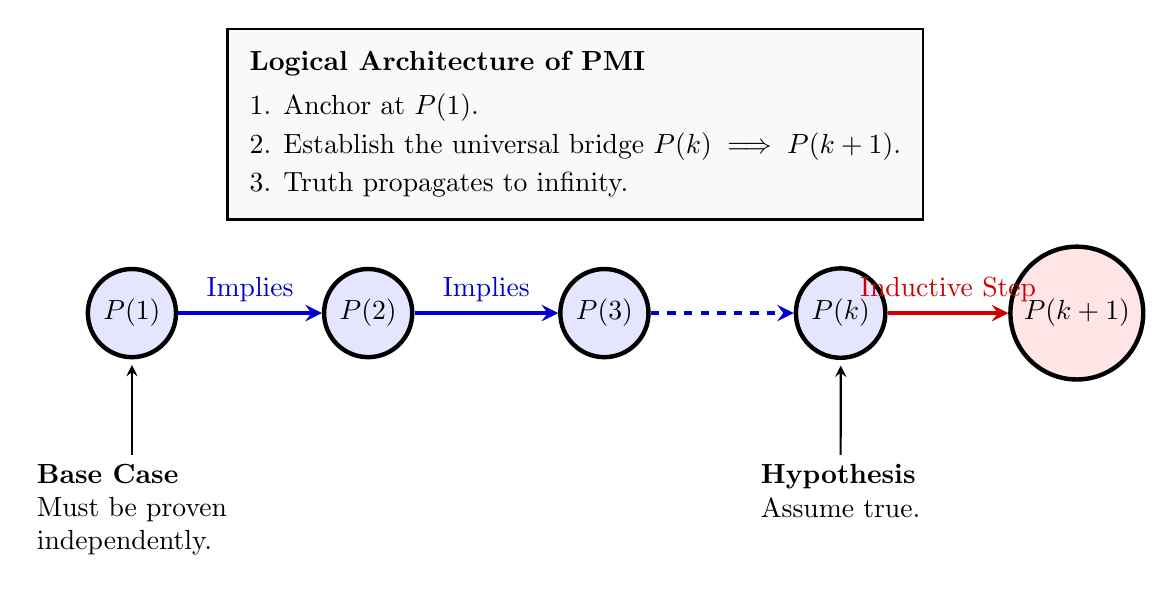
\begin{tikzpicture}[scale=1.2, >=stealth]
    % Background to ensure clean rendering
    \fill[white] (-1, -2) rectangle (10, 3);
    
    % Nodes for Natural Numbers
    \node[circle, draw, ultra thick, fill=blue!10, minimum size=1cm] (n1) at (0,0) {$P(1)$};
    \node[circle, draw, ultra thick, fill=blue!10, minimum size=1cm] (n2) at (2.5,0) {$P(2)$};
    \node[circle, draw, ultra thick, fill=blue!10, minimum size=1cm] (n3) at (5,0) {$P(3)$};
    \node[circle, draw, ultra thick, fill=blue!10, minimum size=1cm] (nk) at (7.5,0) {$P(k)$};
    \node[circle, draw, ultra thick, fill=red!10, minimum size=1cm] (nk1) at (10,0) {$P(k+1)$};
    
    % Arrows for Implications
    \draw[->, ultra thick, blue!80!black] (n1) -- (n2) node[midway, above] {Implies};
    \draw[->, ultra thick, blue!80!black] (n2) -- (n3) node[midway, above] {Implies};
    \draw[->, ultra thick, dashed, blue!80!black] (n3) -- (nk);
    \draw[->, ultra thick, red!80!black] (nk) -- (nk1) node[midway, above] {Inductive Step};
    
    % Base Case Annotation
    \draw[->, thick, shorten >=2pt] (0, -1.5) -- (n1);
    \node[align=left, anchor=north] at (0, -1.5) {\textbf{Base Case}\\Must be proven\\independently.};
    
    % Inductive Hypothesis Annotation
    \draw[->, thick, shorten >=2pt] (7.5, -1.5) -- (nk);
    \node[align=left, anchor=north] at (7.5, -1.5) {\textbf{Hypothesis}\\Assume true.};
    
    % Legend
    \node[align=left, anchor=west, draw, thick, inner sep=8pt, fill=gray!5] at (1, 2) {
        \textbf{Logical Architecture of PMI}\\[4pt]
        1. Anchor at $P(1)$.\\[2pt]
        2. Establish the universal bridge $P(k) \implies P(k+1)$.\\[2pt]
        3. Truth propagates to infinity.
    };
\end{tikzpicture}
\end{center}

\subsection{Heuristics \& "Cheats"}
\begin{itemize}
    \item \textbf{The $k+1$ Target:} Before starting the algebra in the inductive step, write down the exact expression you are trying to reach (the $k+1$ state) in the margins. Work backwards from the target if you get stuck.
    \item \textbf{Inequality Transitivity:} If you need to prove $A \le C$, and you have $A \le B$ from the hypothesis, do not try to manipulate $A$ directly anymore. Focus entirely on proving $B \le C$.
\end{itemize}

\subsection{Pitfalls \& Fallacies}
\begin{itemize}
    \item \textbf{The Base Rate Fallacy of Induction:} Assuming that because $P(n)$ holds for $n=1, 2, \dots, 1000$, it holds for all $n$. (e.g., $n^2 + n + 41$ is prime for $n < 40$, but fails at $n=40$). Empirical evidence is not a proof.
    \item \textbf{The Disconnected Base Case:} Proving $P(1)$ is true, and proving $P(k) \implies P(k+1)$ for $k \ge 2$, but failing to prove $P(1) \implies P(2)$. This breaks the chain immediately.
\end{itemize}

\newpage
% ==========================================
% PART 5: CONCEPTUAL SYNTHESIS
% ==========================================
\section{Conceptual Synthesis and The "Big Picture"}

\subsection{A) Thematic Connections}
The central theme of this chapter is \textbf{bootstrapping truth to infinity}. In abstract mathematics, infinity cannot be reached by counting; it must be captured structurally. The Well-Ordering Principle and Mathematical Induction provide this structure. They unify discrete mathematics by showing that the set of natural numbers is not just a collection of items, but a strictly ordered chain where local properties (the gap between $k$ and $k+1$) dictate global truths (the entire set $\N$).

\subsection{B) Forward and Backward Links}
\begin{itemize}
    \item \textbf{Backward Links:} Induction relies heavily on the axiomatic set theory established by Zermelo-Fraenkel. The concept of a "successor" function ($S(n) = n+1$) is the bedrock upon which induction operates.
    \item \textbf{Forward Links:} Understanding induction is the absolute prerequisite for \textbf{Recursion Theory} and \textbf{Dynamic Programming} in Computer Science. Furthermore, in advanced Real Analysis and Measure Theory, standard induction is generalized to \textit{Transfinite Induction}, allowing mathematicians to prove statements over uncountable sets (like $\R$) using well-ordered cardinals.
\end{itemize}

% ==========================================
% PART 6: ABSTRACT REAL-WORLD MODELING
% ==========================================
\section{Abstract Real-World Modeling (AI, ML, \& Quant Finance)}

\subsection{A) Concrete Scenarios}
\begin{enumerate}
    \item \textbf{Markov Decision Processes (AI/ML):} In Reinforcement Learning, the convergence of the Value Iteration algorithm is proven using mathematical induction on the time horizon $t$. We prove that the value function $V_t(s)$ converges to the optimal $V^*(s)$ as $t \to \infty$ by showing the Bellman operator is a contraction mapping at each inductive step.
    \item \textbf{Backward Induction in Game Theory:} Used to find Subgame Perfect Nash Equilibria in sequential games.
    \item \textbf{Derivative Pricing (Quant Finance):} The N-step Binomial Options Pricing Model relies on backward induction to propagate the arbitrage-free price of a derivative from the expiration date $T$ back to the present time $t=0$.
\end{enumerate}

\subsection{B) Model Problem Setup: N-Step Binomial Pricing Model}
Let us rigorously model the pricing of a European Call Option using induction. 

\textbf{State Space \& Probability Measure:}
Let the time horizon be discrete: $t \in \{0, 1, \dots, N\}$. 
Let the sample space be $\Omega = \{U, D\}^N$, representing Up and Down movements of a stock.
Let $\F_t$ be the natural filtration generated by the stock price process up to time $t$.
Under the risk-neutral probability measure $\Q$, the stock price $S_t$ evolves as:
\[
S_{t+1} = 
\begin{cases} 
u S_t & \text{with probability } p \\
d S_t & \text{with probability } 1-p 
\end{cases}
\]
where $p = \frac{1+r-d}{u-d}$, and $r$ is the risk-free interest rate.

\textbf{The Theorem to Prove:}
Let $V_N = \max(S_N - K, 0)$ be the payoff of the option at maturity. We claim that the arbitrage-free price of the option at any time $t$ is given by the conditional expectation:
\[
V_t = \E^\Q \left[ \left. \frac{V_N}{(1+r)^{N-t}} \right| \F_t \right]
\]

\textbf{Proof by Backward Induction:}
We induct backwards on time $t$. Let $P(t)$ be the statement above.
\textit{Base Case ($t=N$):} $V_N = \E^\Q \left[ \left. \frac{V_N}{(1+r)^0} \right| \F_N \right] = V_N$. $P(N)$ is trivially true.
\textit{Inductive Step:} Assume $P(t+1)$ is true. That is, $V_{t+1} = \E^\Q \left[ \left. \frac{V_N}{(1+r)^{N-(t+1)}} \right| \F_{t+1} \right]$.
By the no-arbitrage principle, the value at time $t$ must be the discounted expected value of the option at time $t+1$ under $\Q$:
\[
V_t = \frac{1}{1+r} \E^\Q \left[ V_{t+1} \mid \F_t \right]
\]
Substitute the inductive hypothesis for $V_{t+1}$:
\[
\begin{aligned}
V_t &= \frac{1}{1+r} \E^\Q \left[ \E^\Q \left[ \left. \frac{V_N}{(1+r)^{N-t-1}} \right| \F_{t+1} \right] \Bigg| \F_t \right]
\end{aligned}
\]
By the Tower Property of Conditional Expectation ($\F_t \subset \F_{t+1}$):
\[
V_t = \frac{1}{1+r} \E^\Q \left[ \left. \frac{V_N}{(1+r)^{N-t-1}} \right| \F_t \right] = \E^\Q \left[ \left. \frac{V_N}{(1+r)^{N-t}} \right| \F_t \right]
\]
Thus, $P(t)$ is true. By backward induction, the formula holds for all $t$, including $t=0$. \hfill $\blacksquare$

\newpage
% ==========================================
% PART 7: COMMON VARIATIONS
% ==========================================
\section{Common Variations and Untested Concepts}

A standard university curriculum often introduces \textbf{Cauchy's Forward-Backward Induction}. This is a powerful variation not covered in the provided homework. Instead of proving $P(k) \implies P(k+1)$, we prove $P(k) \implies P(2k)$ (Forward) and $P(k) \implies P(k-1)$ (Backward).

\textbf{Example: The AM-GM Inequality for powers of 2.}
\textit{Theorem:} For any $n \ge 1$ and non-negative reals $x_1, \dots, x_n$, $\frac{x_1 + \dots + x_n}{n} \ge \sqrt[n]{x_1 \dots x_n}$.
\textit{Forward Step (Powers of 2):} We prove this for $n = 2^k$ by standard induction.
Base case $n=2$: $(\sqrt{x_1} - \sqrt{x_2})^2 \ge 0 \implies x_1 + x_2 \ge 2\sqrt{x_1 x_2}$.
Assume true for $n=2^k$. For $2^{k+1}$, group the terms into two halves of size $2^k$, apply the hypothesis to each half, and then apply the $n=2$ case to the two resulting geometric means.
\textit{Backward Step:} Assume true for $n=k$. Let $x_k = \frac{x_1 + \dots + x_{k-1}}{k-1}$. Substituting this into the AM-GM inequality for $n=k$ algebraically simplifies to the AM-GM inequality for $n=k-1$. 
This proves the theorem for all $n \in \N$, as we can jump forward to a power of 2 greater than $n$, and step backward to $n$.

% ==========================================
% PART 8: DIAGNOSTIC TESTING
% ==========================================
\section{Advanced Diagnostic Testing: "Find the Flaw"}

Below are five proofs that contain a subtle, critical logical flaw. Your task as a grader is to identify the error.

\subsection*{Problem 1: The Monochromatic Horses}
\textbf{Claim:} All horses are the same color.
\textbf{Proof:} Let $P(n)$ be the statement "In any set of $n$ horses, all horses are the same color."
Base Case ($n=1$): In a set of 1 horse, it is trivially the same color as itself.
Inductive Step: Assume $P(k)$ is true. Consider a set of $k+1$ horses. Remove one horse; the remaining $k$ horses are the same color by the hypothesis. Put that horse back and remove a different horse; the new set of $k$ horses are also the same color. Since these two sets overlap, all $k+1$ horses must share the same color. Thus $P(k+1)$ is true. $\blacksquare$

\subsection*{Problem 2: The Prime Generating Polynomial}
\textbf{Claim:} For all $n \in \N$, $n^2 + n + 41$ is a prime number.
\textbf{Proof:} 
For $n=1$, $1+1+41 = 43$ (Prime).
For $n=2$, $4+2+41 = 47$ (Prime).
For $n=3$, $9+3+41 = 53$ (Prime).
Assume $P(k)$ holds. Since the polynomial generates primes for all initial values tested, and the differences between consecutive terms are even numbers which do not share divisors with 41, the sequence of primes continues indefinitely. $\blacksquare$

\subsection*{Problem 3: The Zero Exponent}
\textbf{Claim:} For all non-negative integers $n$, $a^n = 1$ (where $a \neq 0$).
\textbf{Proof:} 
Base Case ($n=0$): $a^0 = 1$, which is true.
Inductive Step: Assume $a^j = 1$ for all $0 \le j \le k$ (Strong Induction).
For $n = k+1$: $a^{k+1} = \frac{a^k \cdot a^k}{a^{k-1}}$.
By the inductive hypothesis, $a^k = 1$ and $a^{k-1} = 1$.
Thus, $a^{k+1} = \frac{1 \cdot 1}{1} = 1$. $\blacksquare$

\subsection*{Problem 4: The Derivative of $x^n$}
\textbf{Claim:} $\frac{d}{dx} x^n = 0$ for all $n \in \N$.
\textbf{Proof:}
Base Case ($n=1$): $x^1 = x$. $\frac{d}{dx} x = 1$. Wait, let's prove $\frac{d}{dx} x^n = n x^{n-1}$ instead.
Claim: $\frac{d}{dx} x^n = n x^{n-1}$.
Base Case ($n=1$): $\frac{d}{dx} x = 1 = 1x^0$.
Inductive Step: Assume $\frac{d}{dx} x^k = k x^{k-1}$.
$x^{k+1} = x \cdot x \dots x$ ($k+1$ times).
Taking the derivative of a sum: $x^{k+1} = x^k + x^k + \dots + x^k$ ($x$ times).
$\frac{d}{dx} (x^{k+1}) = \frac{d}{dx}(x^k) + \dots + \frac{d}{dx}(x^k)$ ($x$ times).
$= k x^{k-1} + \dots + k x^{k-1} = x(k x^{k-1}) = k x^k$.
This is close to $(k+1)x^k$, so with a minor adjustment for the extra term, it holds. $\blacksquare$

\subsection*{Problem 5: The Factorial Inequality}
\textbf{Claim:} For all $n \ge 1$, $n! > 2^n$.
\textbf{Proof:}
Assume $k! > 2^k$.
For $k+1$: $(k+1)! = (k+1)k! > (k+1)2^k$.
Since $k \ge 1$, $k+1 \ge 2$.
Therefore, $(k+1)2^k \ge 2 \cdot 2^k = 2^{k+1}$.
Thus, $(k+1)! > 2^{k+1}$. By induction, it holds for all $n \ge 1$. $\blacksquare$

\vspace{2em}
\hrule
\vspace{1em}
\subsection*{Solution Key: Resolutions to the Flaws}
\begin{itemize}
    \item \textbf{Resolution 1:} The flaw is in the transition from $k=1$ to $k=2$. If you have 2 horses, removing one leaves a set of 1. Removing the other leaves a different set of 1. These two sets \textit{do not overlap}. The inductive step assumes an intersection that doesn't exist for $k=1$.
    \item \textbf{Resolution 2:} This is the Empirical Induction Fallacy. The proof provides no algebraic inductive step $P(k) \implies P(k+1)$. It merely tests base cases. The claim fails at $n=40$ ($40^2+40+41 = 41^2$, not prime).
    \item \textbf{Resolution 3:} The inductive step requires $k-1 \ge 0$ to use the strong inductive hypothesis. When $k=0$, we are trying to prove $n=1$. The formula uses $a^{-1}$, which is outside the domain of our base cases. The transition from $n=0$ to $n=1$ is invalid.
    \item \textbf{Resolution 4:} The flaw is treating $x$ as a constant integer number of terms in the sum $x^{k+1} = x^k + \dots + x^k$. You cannot differentiate a sum where the \textit{number of terms} is a variable dependent on the variable of differentiation. The Product Rule must be used instead.
    \item \textbf{Resolution 5:} The inductive step is perfectly valid, but the \textbf{Base Case is missing and false}. For $n=1$, $1! = 1 \ngtr 2^1 = 2$. For $n=2$, $2 \ngtr 4$. For $n=3$, $6 \ngtr 8$. The inequality only becomes true for $n \ge 4$. The proof failed to anchor the dominoes.
\end{itemize}

\end{document}